\chapter{Xây dựng và Triển khai Ứng dụng}
\label{chap:deployment}

\section{Kiến trúc hệ thống}
Ứng dụng được xây dựng theo kiến trúc web ba lớp: frontend React/Vite, backend Node.js--Express theo mô hình MVC và dịch vụ mô hình RAG chạy tách biệt. Cách tách này giúp giao diện, nghiệp vụ, cơ sở dữ liệu và mô hình học máy có thể phát triển độc lập; khi URL hoặc cách triển khai mô hình thay đổi, nhóm chỉ cần cập nhật cấu hình backend thay vì sửa toàn bộ ứng dụng.

\begin{table}[H]
\centering
\caption{Các thành phần chính của hệ thống}
\label{tab:deployment-components}
\begin{tabularx}{\textwidth}{p{3.4cm}Y}
\toprule
\textbf{Thành phần} & \textbf{Vai trò}\\
\midrule
Frontend & React/Vite, hiển thị giao diện đăng nhập, sidebar lịch sử, khung chat, nguồn tham khảo và liên kết bản đồ.\\
Backend & Express MVC, xử lý xác thực, hội thoại, tin nhắn, tích hợp RAG API và SSE.\\
Database & SQLite, lưu người dùng, hội thoại, tin nhắn và metadata nguồn tham khảo.\\
RAG API & Dịch vụ suy luận riêng, nhận câu hỏi và trả về câu trả lời kèm nguồn.\\
\bottomrule
\end{tabularx}
\end{table}

Backend được chia thành các lớp \texttt{routes}, \texttt{controllers}, \texttt{services} và \texttt{models}. Các bảng chính gồm \texttt{users}, \texttt{conversations}, \texttt{messages} và \texttt{medical\_sources}. Trường \texttt{user\_id} trong bảng \texttt{conversations} giúp mỗi tài khoản chỉ truy cập được lịch sử của chính mình.

\section{Tích hợp mô hình}
Mô hình RAG không được nhúng trực tiếp vào Node.js mà được gọi qua HTTP API bằng lớp \texttt{RagApiService}. Frontend gửi câu hỏi đến backend qua \texttt{POST /api/chat} hoặc \texttt{POST /api/chat/stream}; backend kiểm tra token, lưu câu hỏi, gọi RAG API với \texttt{query} và \texttt{session\_id}, sau đó lưu câu trả lời vào SQLite.

Để tạo cảm giác realtime, endpoint \texttt{/api/chat/stream} sử dụng Server-Sent Events. Các sự kiện chính gồm \texttt{conversation}, \texttt{status}, \texttt{token}, \texttt{done} và \texttt{error}. Khi RAG API lỗi hoặc timeout, backend vẫn lưu câu hỏi và trả về thông báo fallback để người dùng biết hệ thống chưa kết nối được với mô hình, tránh làm gián đoạn phiên hội thoại.

\section{Giao diện và chức năng}
Ứng dụng có màn hình đăng nhập/đăng ký trước khi vào chatbot. Mật khẩu được hash bằng PBKDF2 kèm salt riêng; sau khi đăng nhập, backend cấp Bearer token để frontend gửi kèm trong các request tiếp theo. Các API hội thoại đều đi qua middleware xác thực, nhờ đó dữ liệu lịch sử được tách theo từng người dùng.

Các chức năng chính đã hoàn thiện gồm:
\begin{itemize}
    \item Đăng ký, đăng nhập, đăng xuất và lưu phiên người dùng.
    \item Tạo, chọn lại, đổi tên và xóa cuộc trò chuyện.
    \item Gửi câu hỏi y tế tiếng Việt và nhận câu trả lời realtime bằng SSE.
    \item Hiển thị nguồn tham khảo nếu RAG API trả về.
    \item Mở Google Maps để gợi ý bệnh viện, phòng khám hoặc nhà thuốc gần vị trí hiện tại.
    \item Hiển thị cảnh báo rằng nội dung chỉ mang tính tham khảo, không thay thế tư vấn của bác sĩ.
\end{itemize}

Giao diện chính được thiết kế theo dạng dashboard y tế tối giản. Sidebar nằm bên trái, chứa thông tin tài khoản, nút tạo hội thoại mới, lịch sử trò chuyện và nhóm liên kết bản đồ. Khung chat nằm bên phải, trong đó vùng tin nhắn có thanh cuộn riêng còn ô nhập câu hỏi được cố định ở cuối màn hình, giúp người dùng vẫn có thể tiếp tục nhập khi câu trả lời dài.

\begin{figure}[H]
    \centering
    \begin{minipage}{0.49\textwidth}
        \centering
        \IfFileExists{figures/auth-login-screen.png}{
            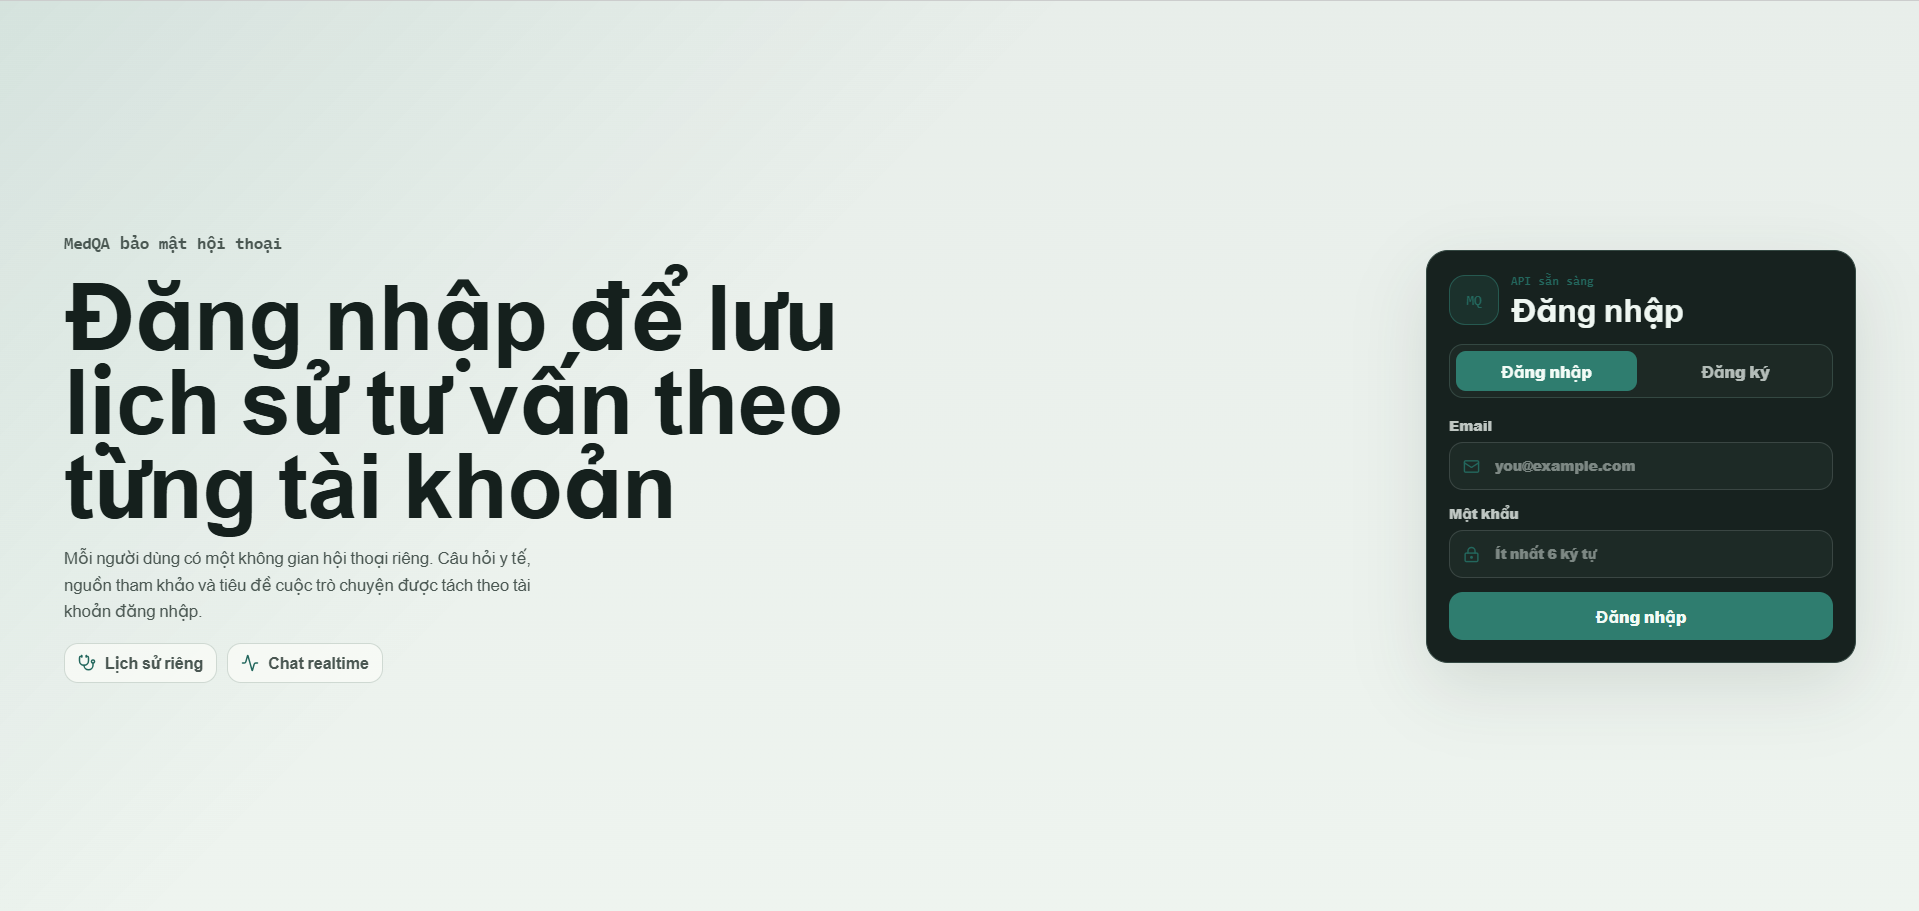
\includegraphics[width=\linewidth]{figures/auth-login-screen.png}
        }{
            \fbox{\parbox[c][3cm][c]{0.95\linewidth}{\centering Chèn ảnh đăng nhập}}
        }
    \end{minipage}
    \hfill
    \begin{minipage}{0.49\textwidth}
        \centering
        \IfFileExists{figures/auth-register-screen.png}{
            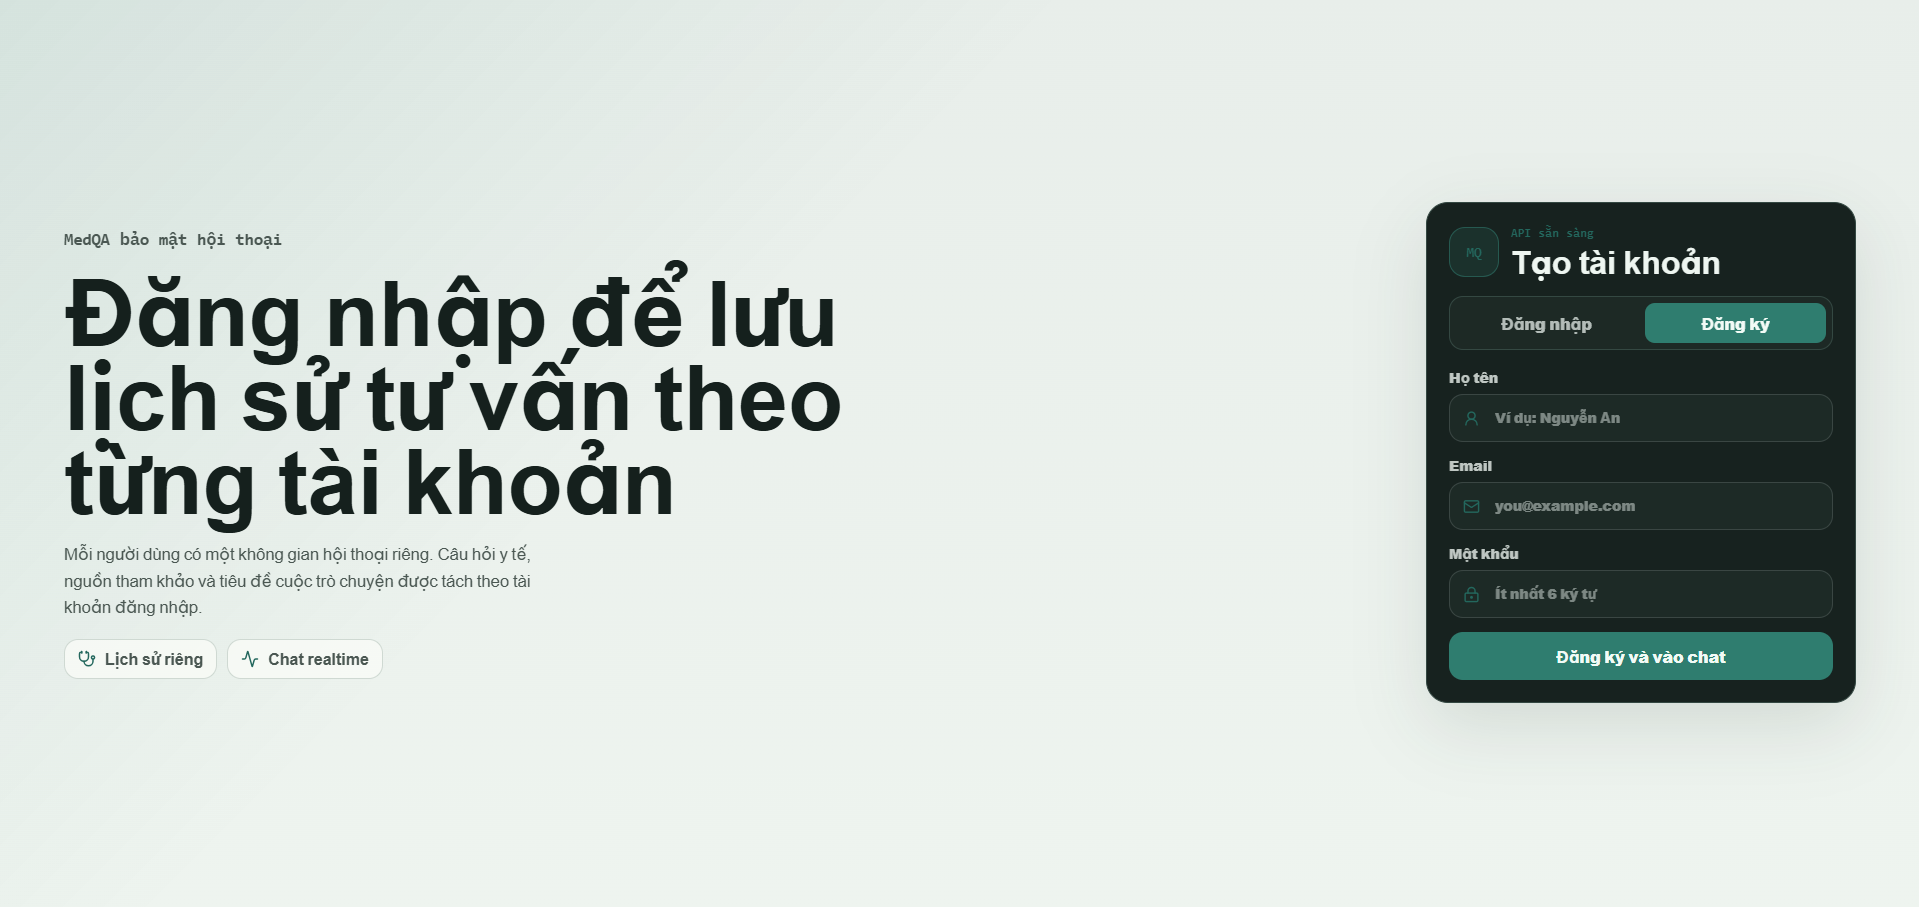
\includegraphics[width=\linewidth]{figures/auth-register-screen.png}
        }{
            \fbox{\parbox[c][3cm][c]{0.95\linewidth}{\centering Chèn ảnh đăng ký}}
        }
    \end{minipage}
    \caption{Màn hình đăng nhập và đăng ký tài khoản.}
    \label{fig:auth-screens}
\end{figure}

\begin{figure}[H]
    \centering
    \IfFileExists{figures/chat-main-screen.png}{
        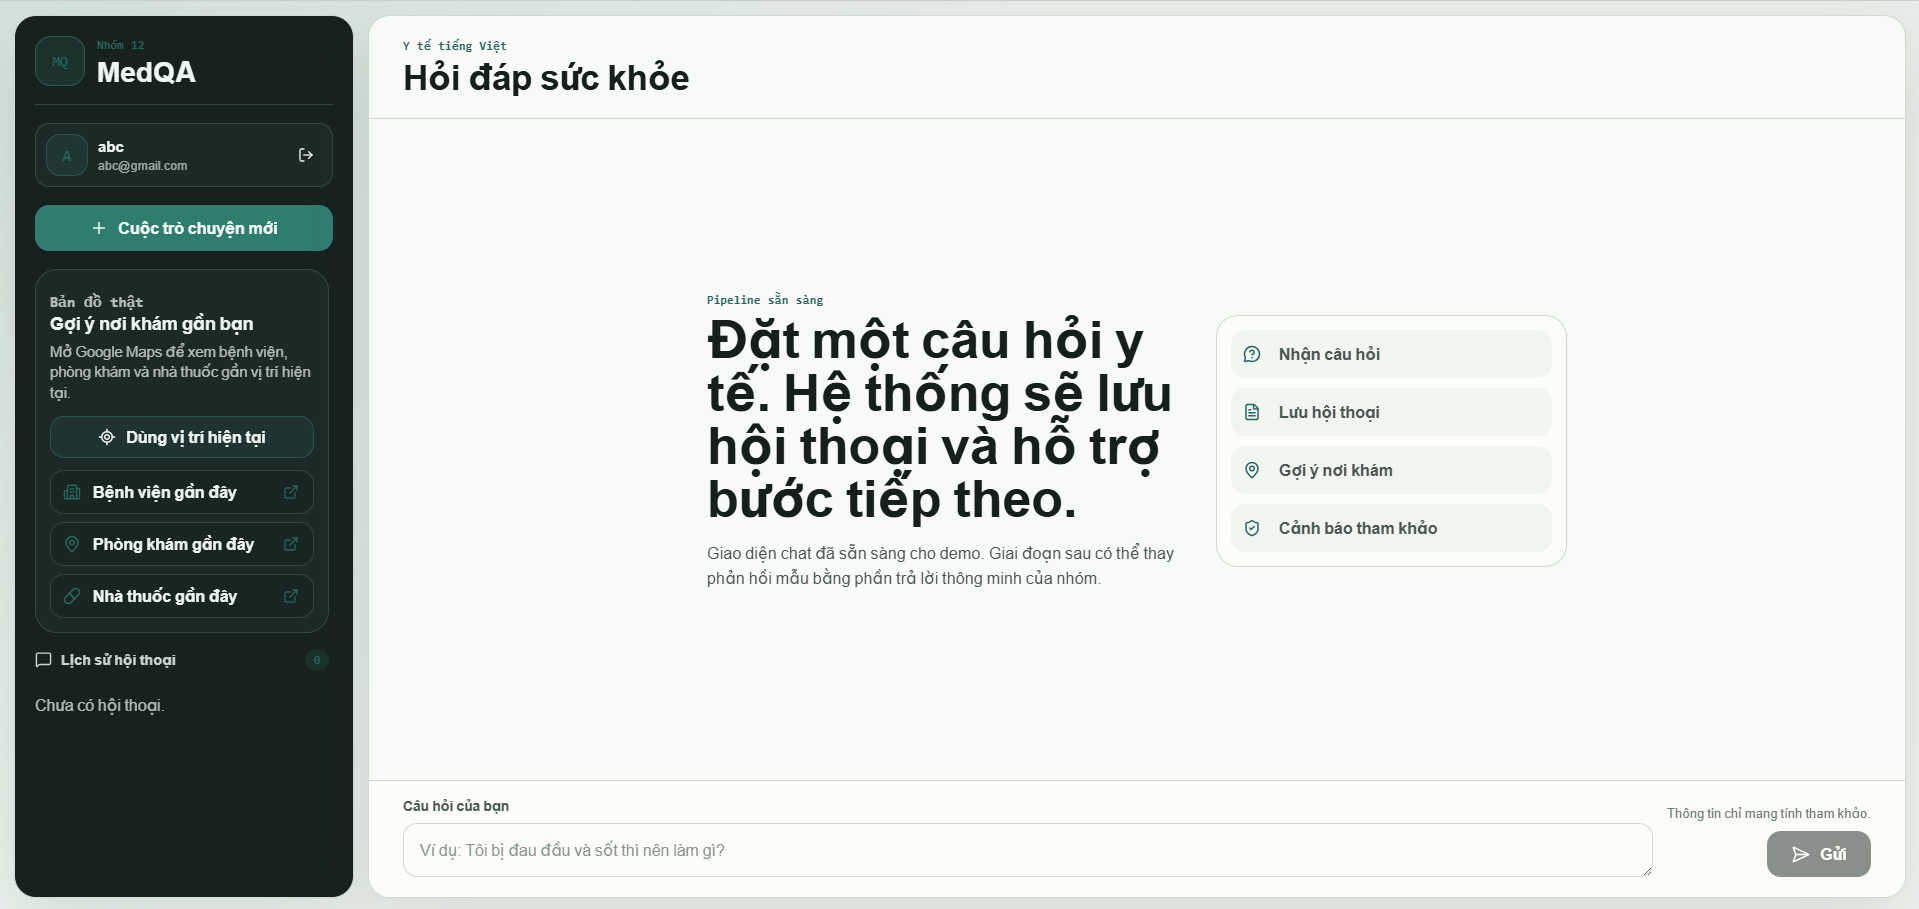
\includegraphics[width=0.86\textwidth]{figures/chat-main-screen.png}
    }{
        \fbox{\parbox[c][4cm][c]{0.86\textwidth}{\centering Chèn ảnh màn hình chatbot}}
    }
    \caption{Giao diện chatbot sau khi đăng nhập.}
    \label{fig:chat-main-screen}
\end{figure}

\begin{figure}[H]
    \centering
    \IfFileExists{figures/nearby-hospitals-screen.png}{
        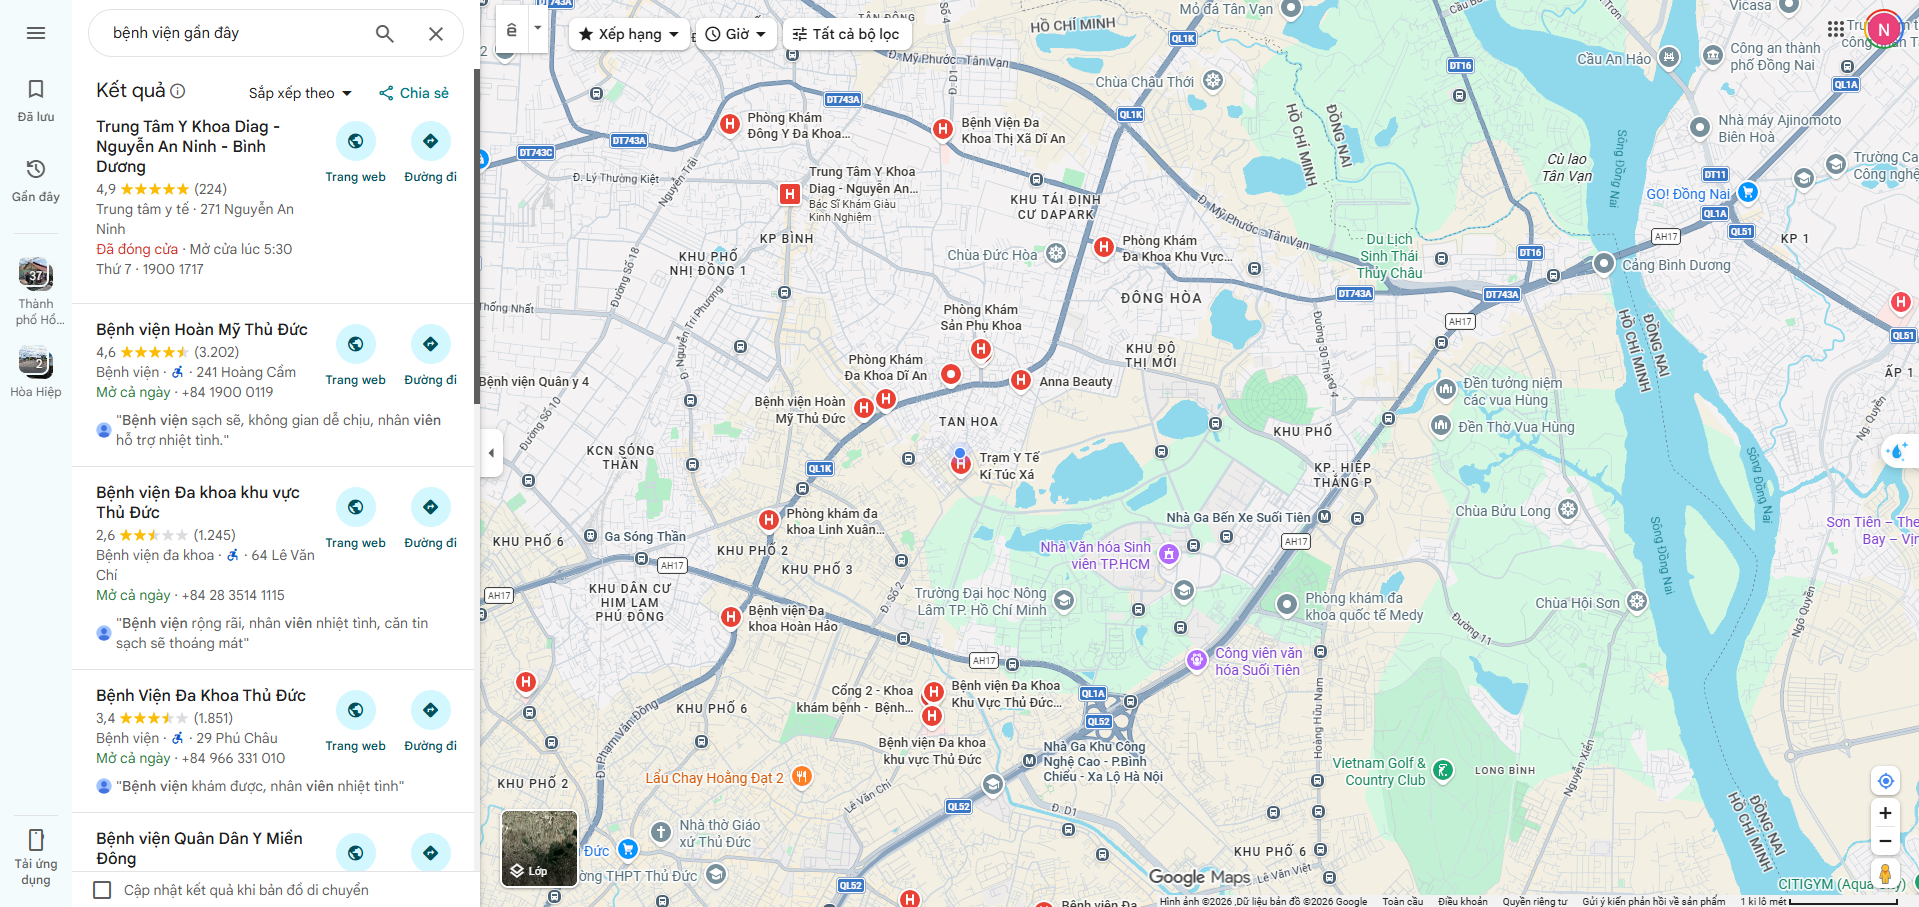
\includegraphics[width=0.86\textwidth]{figures/nearby-hospitals-screen.png}
    }{
        \fbox{\parbox[c][4cm][c]{0.86\textwidth}{\centering Chèn ảnh gợi ý bệnh viện gần đây}}
    }
    \caption{Gợi ý bệnh viện gần đây thông qua Google Maps.}
    \label{fig:nearby-hospitals-screen}
\end{figure}

\section{Triển khai}
Ứng dụng được triển khai trên VPS Ubuntu bằng PM2. Frontend và backend chạy thành hai tiến trình riêng, tránh ảnh hưởng đến các dịch vụ khác trên máy chủ. SQLite được đặt trong thư mục dùng chung để khi cập nhật mã nguồn, dữ liệu người dùng và lịch sử hội thoại không bị mất.

\begin{itemize}
    \item Repository: \url{https://github.com/Nguyennnm/ML-CHATBOT_MEDICAL}
    \item Frontend: \url{http://84.247.147.180:18180}
    \item Backend health check: \url{http://84.247.147.180:18181/api/health}
    \item Database: \texttt{/opt/ml-web/shared/medical\_chatbot.sqlite}
\end{itemize}

Khi chạy local, nhóm cài dependency bằng \texttt{npm install}, chạy migration bằng \texttt{npm run db:migrate} và khởi động frontend/backend bằng \texttt{npm run dev}. Các biến môi trường quan trọng gồm \texttt{PORT}, \texttt{CLIENT\_ORIGIN}, \texttt{DB\_PATH}, \texttt{RAG\_API\_BASE\_URL}, \texttt{AUTH\_TOKEN\_SECRET} và \texttt{AUTH\_TOKEN\_TTL\_SECONDS}.

\section{Kiểm thử và vận hành}
Nhóm đã kiểm thử các luồng chính: đăng ký, đăng nhập, tạo hội thoại, đổi tên, xóa hội thoại, gửi câu hỏi, stream câu trả lời và hiển thị nguồn tham khảo. Với phần phân quyền, hai tài khoản khác nhau được dùng để kiểm tra rằng người dùng không thể xem hoặc truy cập trực tiếp hội thoại của tài khoản khác. API \texttt{/api/conversations} trả \texttt{401} khi thiếu token và trả \texttt{404} khi truy cập hội thoại không thuộc người dùng hiện tại.

Sau khi triển khai, frontend public trả mã \texttt{200}, backend health check trả \texttt{\{"status":"ok"\}}, và hai tiến trình \texttt{ml-web-api}, \texttt{ml-web-client} hoạt động ổn định trên PM2. Ở mức đồ án, hệ thống đã có các biện pháp bảo mật cơ bản như hash mật khẩu, Bearer token, kiểm soát CORS, giới hạn độ dài tin nhắn và tách dữ liệu theo \texttt{user\_id}. Nếu triển khai thực tế, hệ thống nên bổ sung HTTPS, domain, reverse proxy, rate limiting và cơ chế backup cơ sở dữ liệu.

\section{Kết luận chương}
Chương này trình bày phiên bản web của hệ thống hỏi--đáp y tế tiếng Việt. Sản phẩm đã có giao diện React, backend Express MVC, cơ sở dữ liệu SQLite, xác thực người dùng, quản lý lịch sử hội thoại, trả lời realtime bằng SSE, liên kết bản đồ gợi ý cơ sở y tế và triển khai public trên VPS. Đây là nền tảng để nhóm tiếp tục hoàn thiện chất lượng mô hình RAG và mở rộng hệ thống trong các giai đoạn sau.
